%!TEX root = ../main.tex 
\section{How harder are rotting bandits ?}
\label{sec:howhard}
In the last sections, we presented \RAWUCB, an algorithm which extends the results of \UCBone \citep{auer2002finite} on stationary bandits to the more general rotting bandits setup. Hence, we conclude that rotting bandits are not much harder than stationary ones. 

Yet, \UCBone is only near asymptotic and minimax optimal. In Section~\ref{sec:stoch-bandits}, we explain that a better tuning of the confidence levels allows \UCB variant to match the asymptotic and minimax rates for gaussian bandits.

This section investigates the impact of confidence levels tuning on \RAWUCB. How does it compare with \UCB on stationary bandits?  Does it improve the performance of \RAWUCB on our rotting benchmarks? 

\subsection{{\RAWUCBpp}}
We introduce \RAWUCBpp, an algorithm which uses the \RAWUCB procedure (Alg.\ref{alg:RAWUCB}) with a new index,
\begin{multline}
\label{eq:rawpp_index}
\operatorname{ind}(i,t, \delta_{t,h}) \triangleq \min_{h\leq N_{i,t-1}}\pa{ {\hmu}_i^h(\Nitmone) + \sqrt{\frac{2\sigma^2\log_+\pa{\nicefrac{2}{\delta_{t,h}}}}{h}}}\\ \text{ with } \; \delta_{t,h} \triangleq \frac{2\pa{\nicefrac{Kh}{t}}^\alpha}{\pa{1+ \log_+\pa{\nicefrac{t}{Kh}}}^\beta}\CommaBin
\end{multline}

with $\log_+\pa{\cdot} \triangleq \max\pa{\log\pa{\cdot}, 0}$. The main difference with the index of \RAWUCB in Equation~\ref{eq:raw_index} is the more complex confidence level. First, we multiply our confidence level by $Kh$ and replace $\log$ by $\log_+$. This is similar to the $\delta = \nicefrac{KN_{i,t}}{t}$ of \MOSSa  \citep{degenne2016anytime}. We replace $N_{i,t}$ - the number of pulls of arm $i$ at the round $t$- by $h$, the number of sample in the associated average. Indeed, let us consider a two-arm bandit problem where the first arm has a much larger value $\mu_2 + 100 \sigma$ than the second one (with value $\mu_2$) at the beginning of the game. Hence, at the beginning of the game, $N_{1,t} \sim t$ because \RAWUCBpp can quickly identify arm $1$ as the current best arm. After $\frac{T}{2}$ pulls, arm $1$ abruptly decay to a value $\mu_2 + \sigma$. If we do not replace $N_{i,t}$ by $h$ in the confidence levels in Equation~\ref{eq:rawpp_index}, the exploration bonus would be canceled until the end of the game for all the UCB of arm $1$ because $\frac{KN_{i,t}}{t} > 1$. Without the exploration bonus, there is a large enough probability that the index of arm $1$ takes a value below $\mu_2$. Indeed, since we take the minimum across indexes, if the first reward sample after the decay is below $\mu_2$, then the meta-index will be below $\mu_2$. In this case, \RAWUCB may pull arm $2$ until the end of the game and suffer at least $\cO\pa{\sigma T}$ regret. Replacing $N_{i,t}$ by $h$ restore the exploration bonus for arms which have recently decay. 

Second, we add a logarithmic exploration inflation factor. Notice that we also divide $t$ by $Kh$ in the inner logarithm, as it is done for \KLUCBpp \citep{menard2017klucb++}. When the noise is not gaussian, the concentration results are slightly less tight and the asymptotic optimality proof often needs this factor. For instance, \citet{cappe2013klucb} use a factor $\log\pa{t}^{-3}$ in their theory, but they recommend to not use it in practice. However, for \RAWUCB, we believe that extra-exploration is needed in practice. Indeed, we find our best experimental performance for $\alpha=1.4$ which is larger than the asymptotic optimal tuning for \UCB $\alpha=1$ \citep{lattimore2020banditbook}. In our theory in Section~\ref{sec:theory}, we increase $\alpha$ by one compared to \UCBone to ensure that the $t$ (instead of $K$) constructed statistics were into the confidence levels. 




\subsection{Experiments}
\subsubsection{Stationary Experiment}

\paragraph{Setup.} We consider a stationary bandits with two arms with $\mu_1= 0$ and $\mu_2 = \Delta$. We consider two different values of $\Delta \in \left\{0.01, 1\right\}$. The rewards are then generated by applying a Gaussian i.i.d.\,noise $\mathcal{N}\left(0,\subgaussian = 1\right)$. We run the experiment with the horizon $T=10^6$.

\paragraph{Algorithms.} We consider \UCB and \MOSSa \citep{degenne2016anytime}. We tune \UCB with asymptotic optimal confidence level $\sqrt{\nicefrac{2\log\pa{t}}{\Nit}}$ \citep{lattimore2020banditbook}. For \MOSSa, we use $\sqrt{\nicefrac{2\log\pa{\nicefrac{t}{K\Nit}}}{\Nit}}$, which corresponds to a tuning of its parameter $\alpha = 3$. We test \RAWUCBpp with many different values, but we display two different sets of values $\alpha = 1$ and $\beta = 3.5$ or $\alpha = 2$ and $\beta=0$. These two sets of values give the most consistent performance on the two problems. We add \RAWUCB with $\alpha = 1.4$ for comparison. For \RAWUCB and \RAWUCBpp , we use the efficient version with $m=1.01$ which performs similarly than the classical algorithm Subsection~\ref{ss:eff-exp}.

\begin{figure*}[ht]
\centering
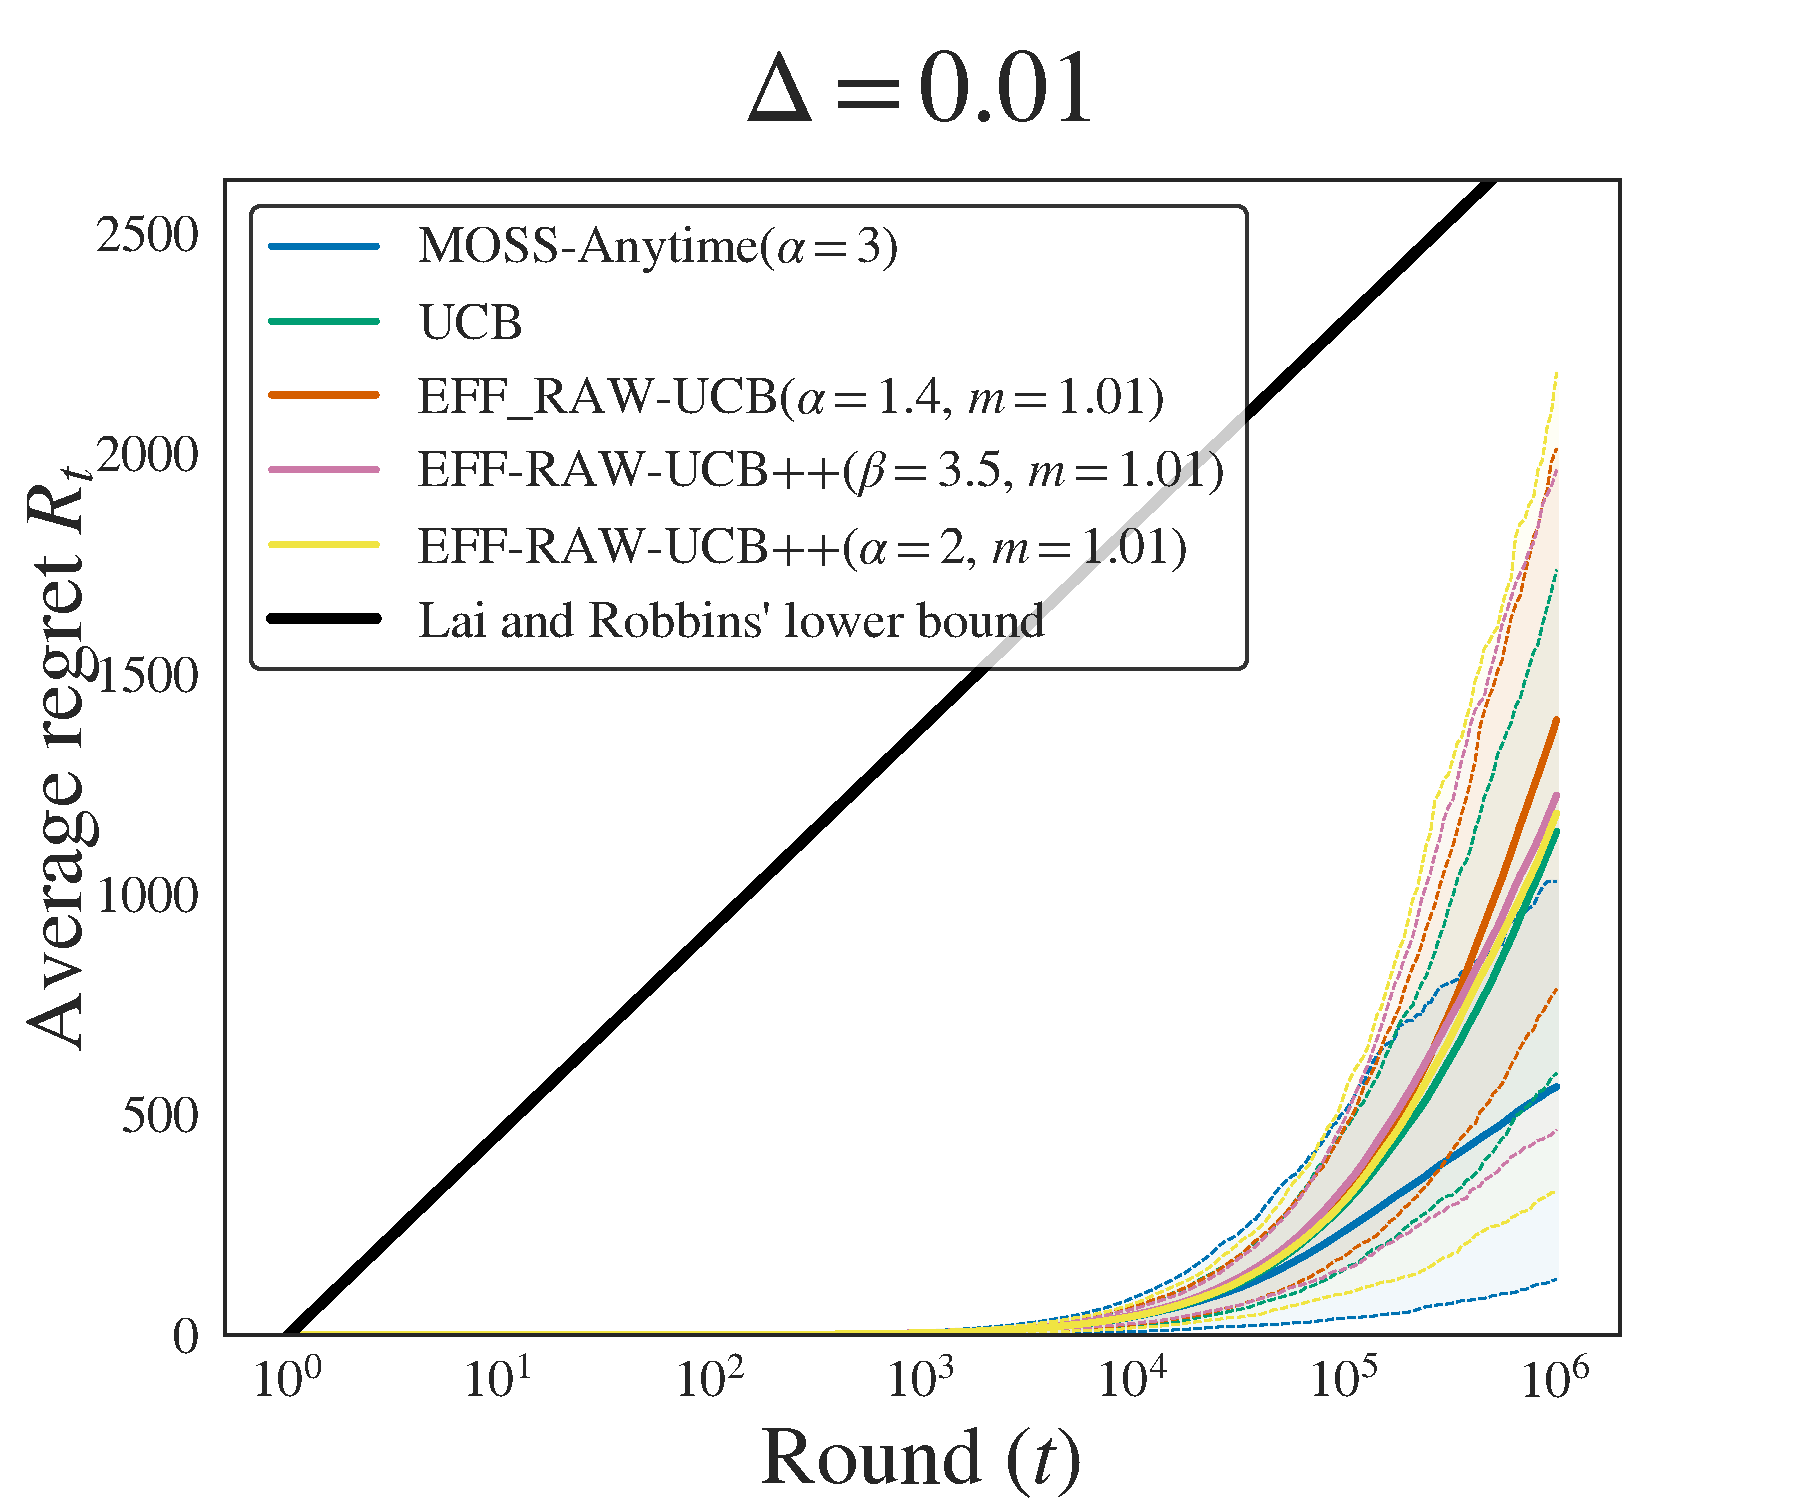
\includegraphics[clip, width= 0.49\textwidth]{2.1Rested/fig/fig_asy0,01.pdf}
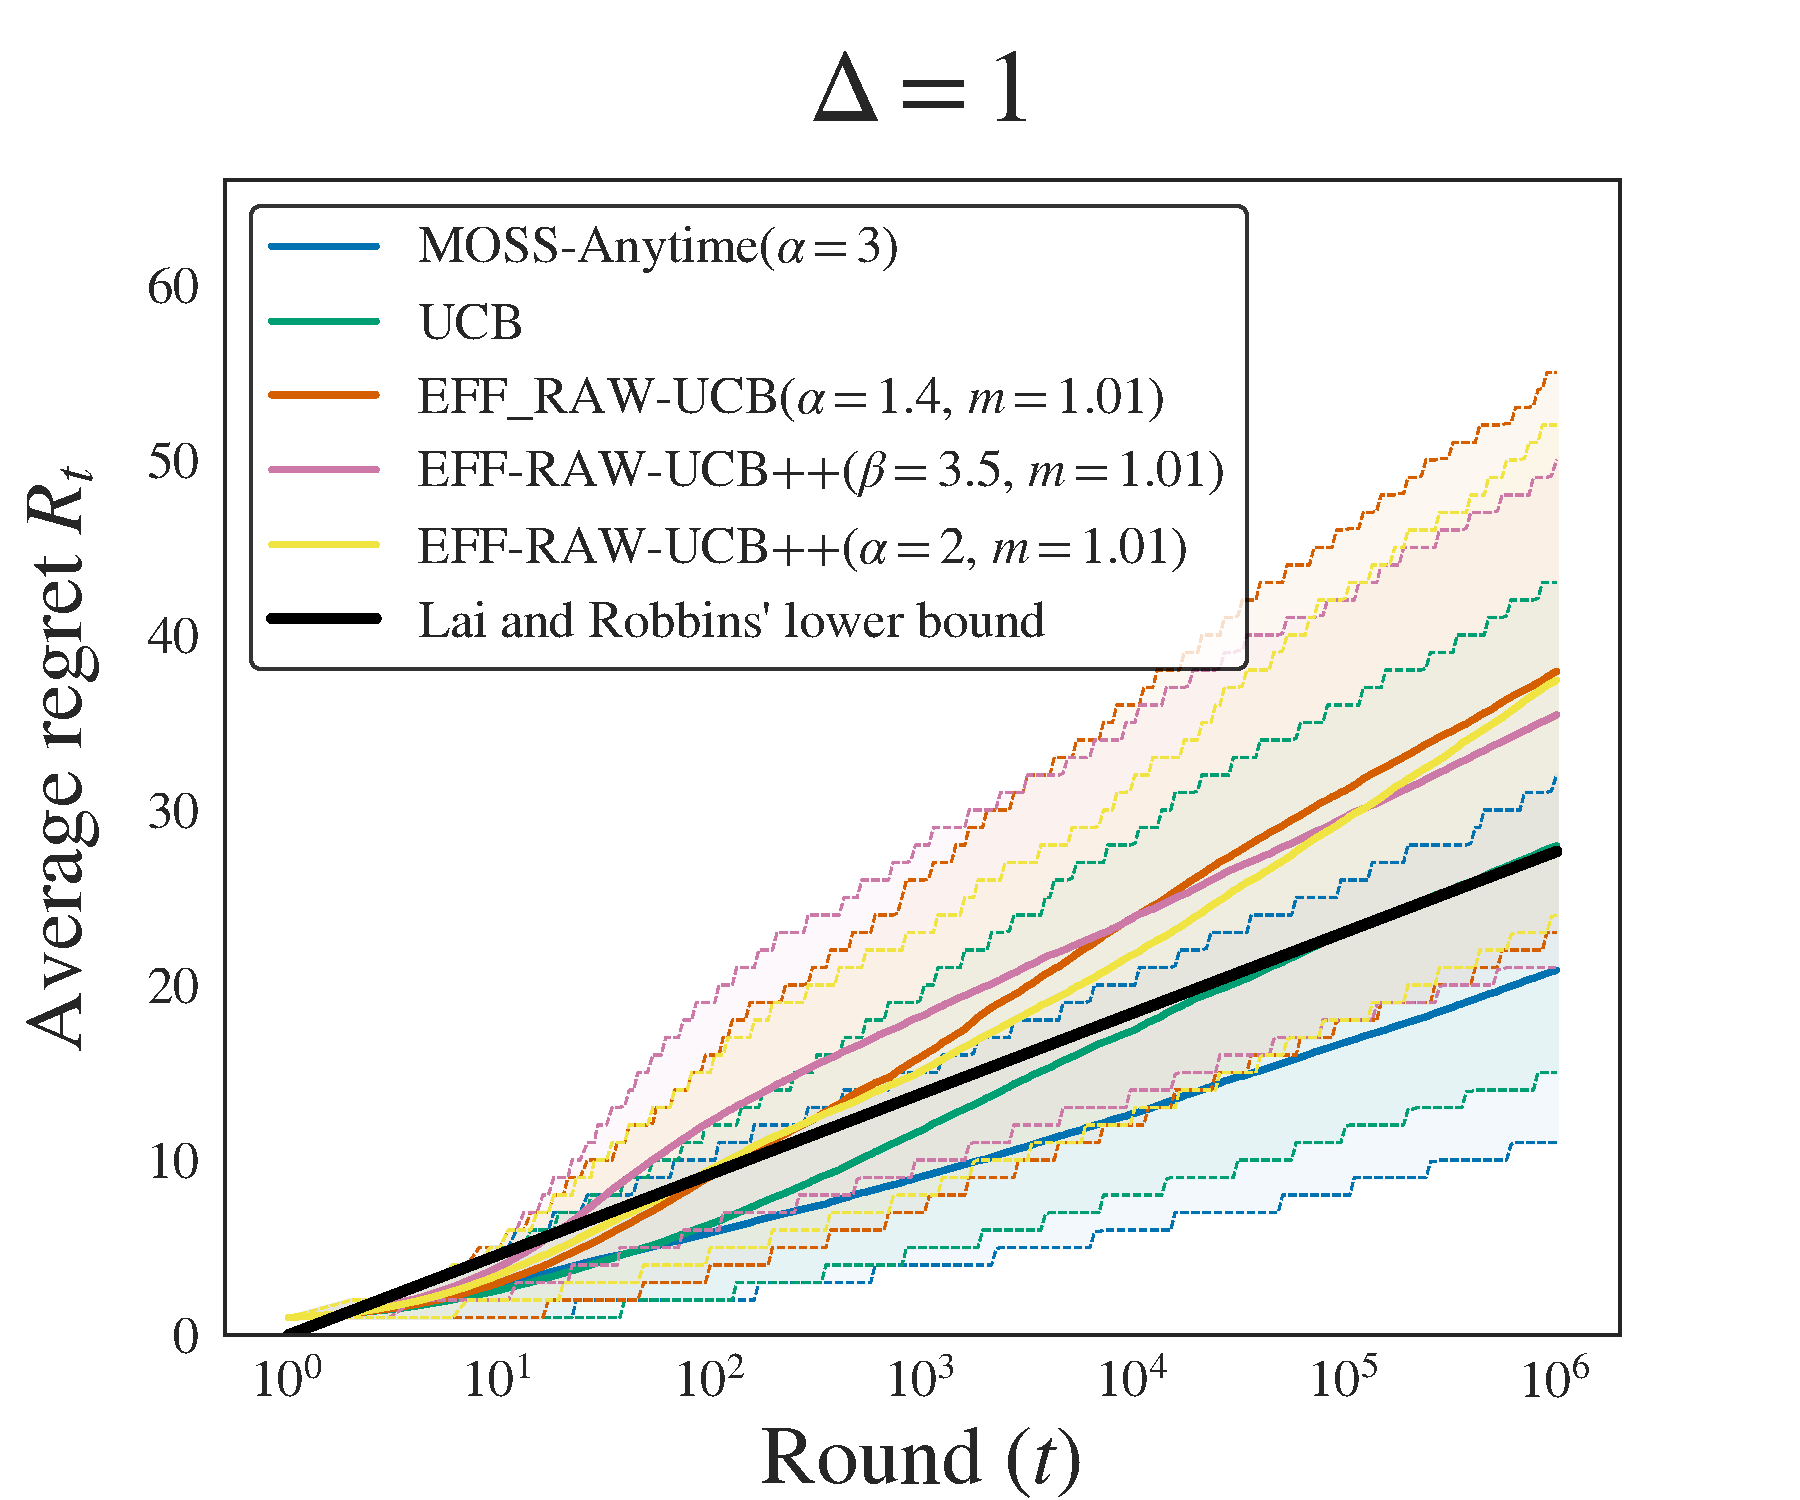
\includegraphics[clip, width= 0.49\textwidth]{2.1Rested/fig/fig_asy1.pdf}
\caption{Stationary experiments}
\label{fig:stationary-experiment}
\end{figure*}
\paragraph{Results.}  \RAWUCBpp seems to improve slightly the results compare to \RAWUCB. Yet, the improvement is not as significant than between \MOSSa and \UCB. On the $\Delta=1$ experiment, we see that the tuning with the logarithm ($\beta=3.5$) seems to enjoy better asymptotic guarantee than the tuning with $\alpha = 2$. Yet, it is not clear if \RAWUCBpp ($\beta=3.5$) is asymptotic optimal with respect to the Lai and Robbin's lower bound. However, at finite horizon, the different parameters are quite close to each other.



\subsubsection{Rotting Experiments $\#$1 (2 arms) and $\#$2 (10 arms).}
\paragraph{Setup and Algorithms.} We study the two benchmarks described in Subsection~\ref{subsec:rested-experiment1} and Section~\ref{sec:rested-experiment}. In Figures~\ref{fig:rested-eff1} and~\ref{fig:rested-eff2}, we compare \EFFRAWpp ($\alpha=2$, $m=1.01$) with \EFFRAW  ($\alpha=1.4$, $m=1.01$). The parameters $\alpha$ were selected according to previous experiments.

\paragraph{Results.} \EFFRAWpp performs slightly better than \EFFRAW for almost any experiments and at almost any rounds. A noticeable exception is when $L$ is large in the two-arms experiment: the result of \EFFRAWpp is slightly worse than for \EFFRAW. Overall, the results suggest that the aggressive confidence tuning technique of stationary bandits also improves the rotting adaptivity. Yet, we notice that the confidence levels with $\alpha =2$ are less tight than the tuning of \MOSSa (which would correspond to $\alpha=1$).

\begin{figure*}[ht]
\centering
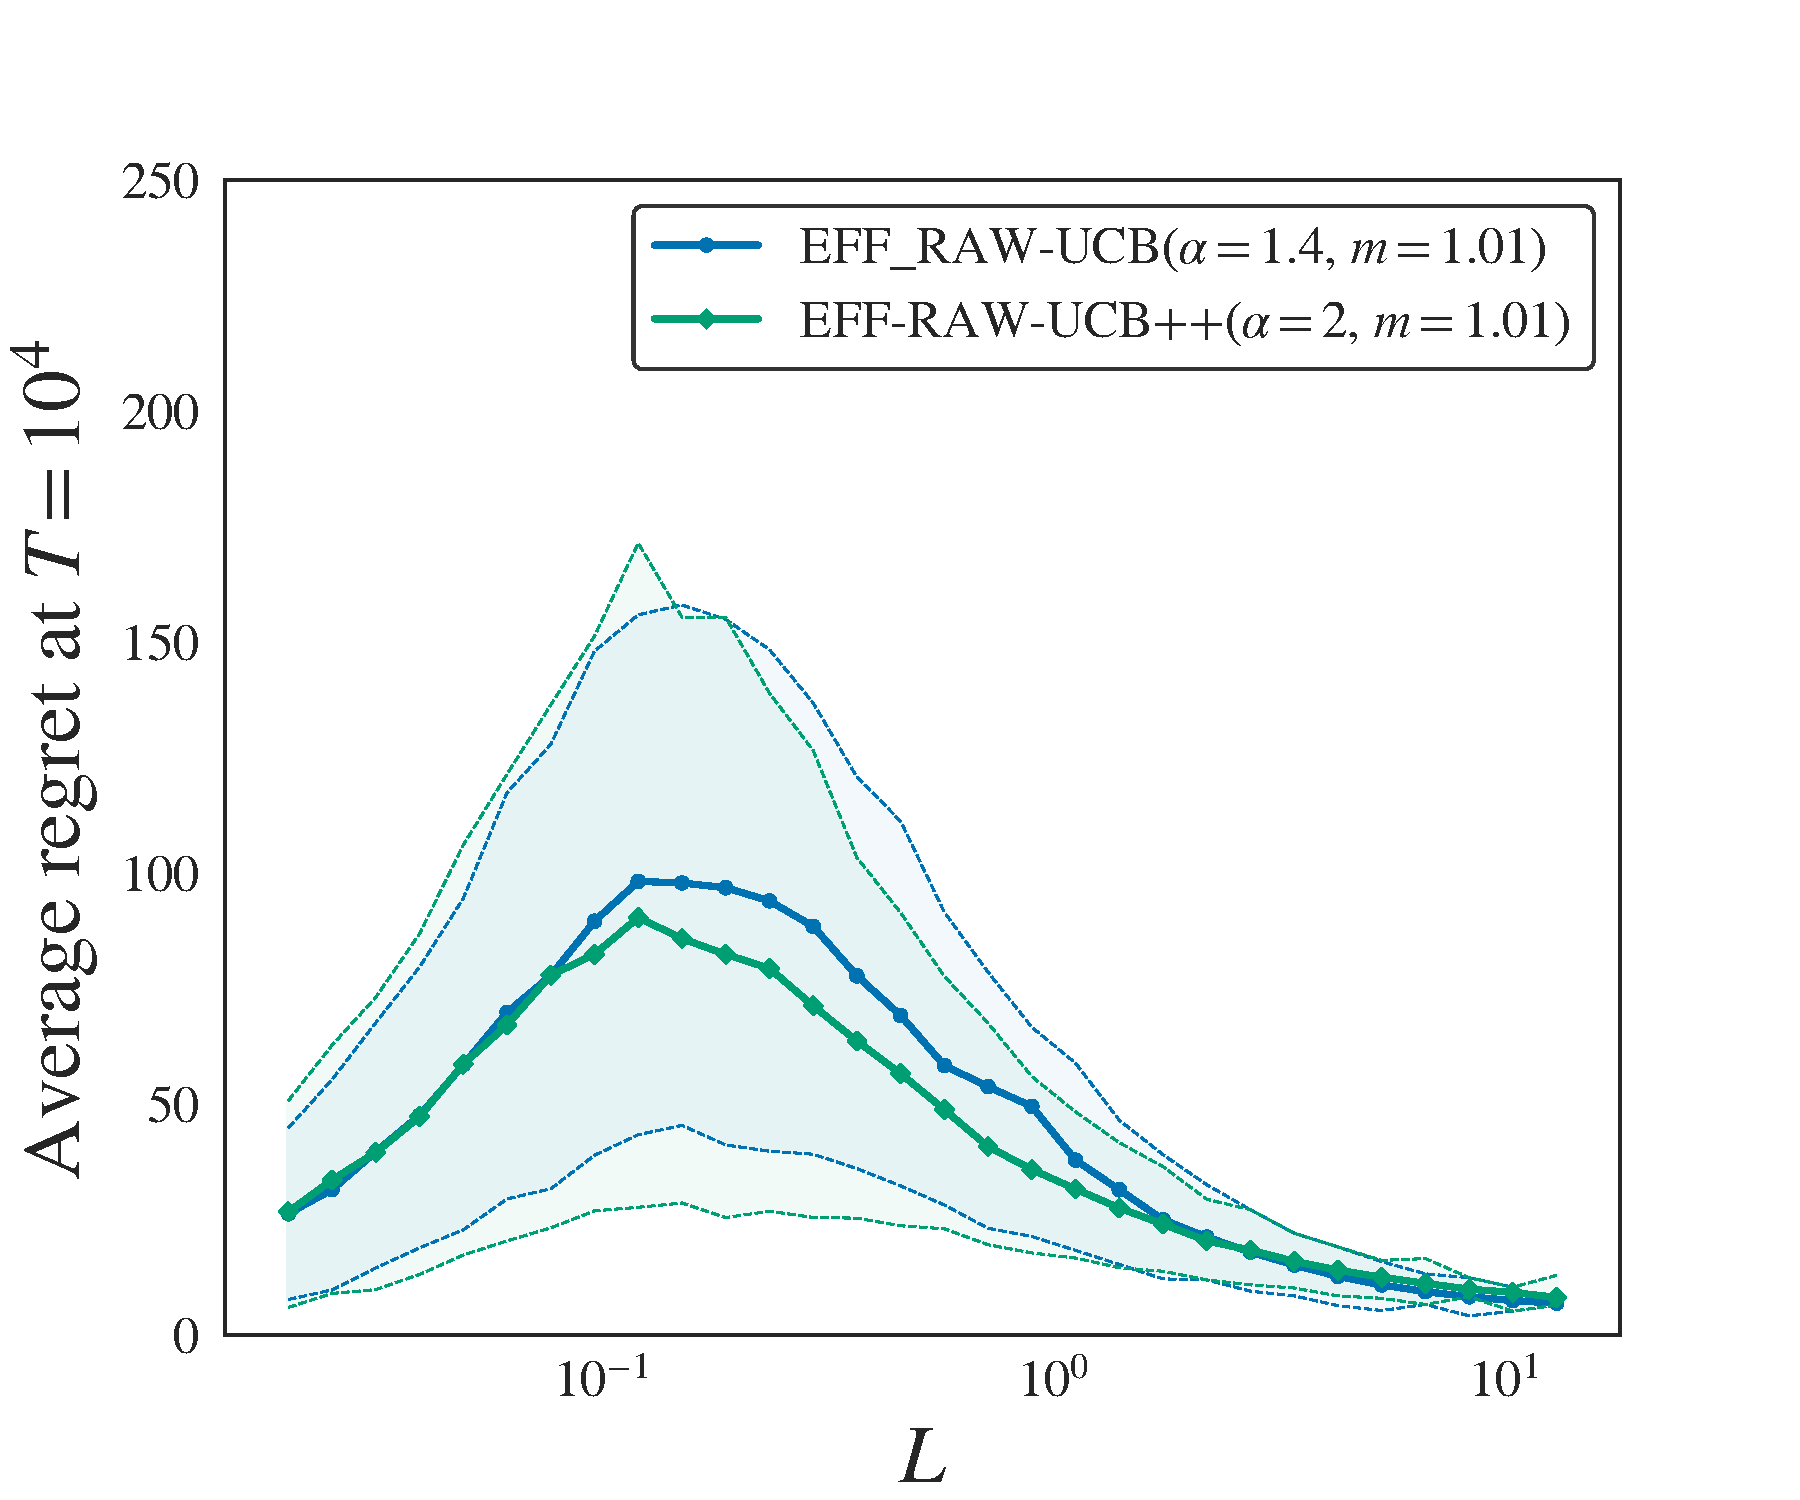
\includegraphics[clip, width= 0.51\textwidth]{2.1Rested/fig/fig1A_pp.pdf}
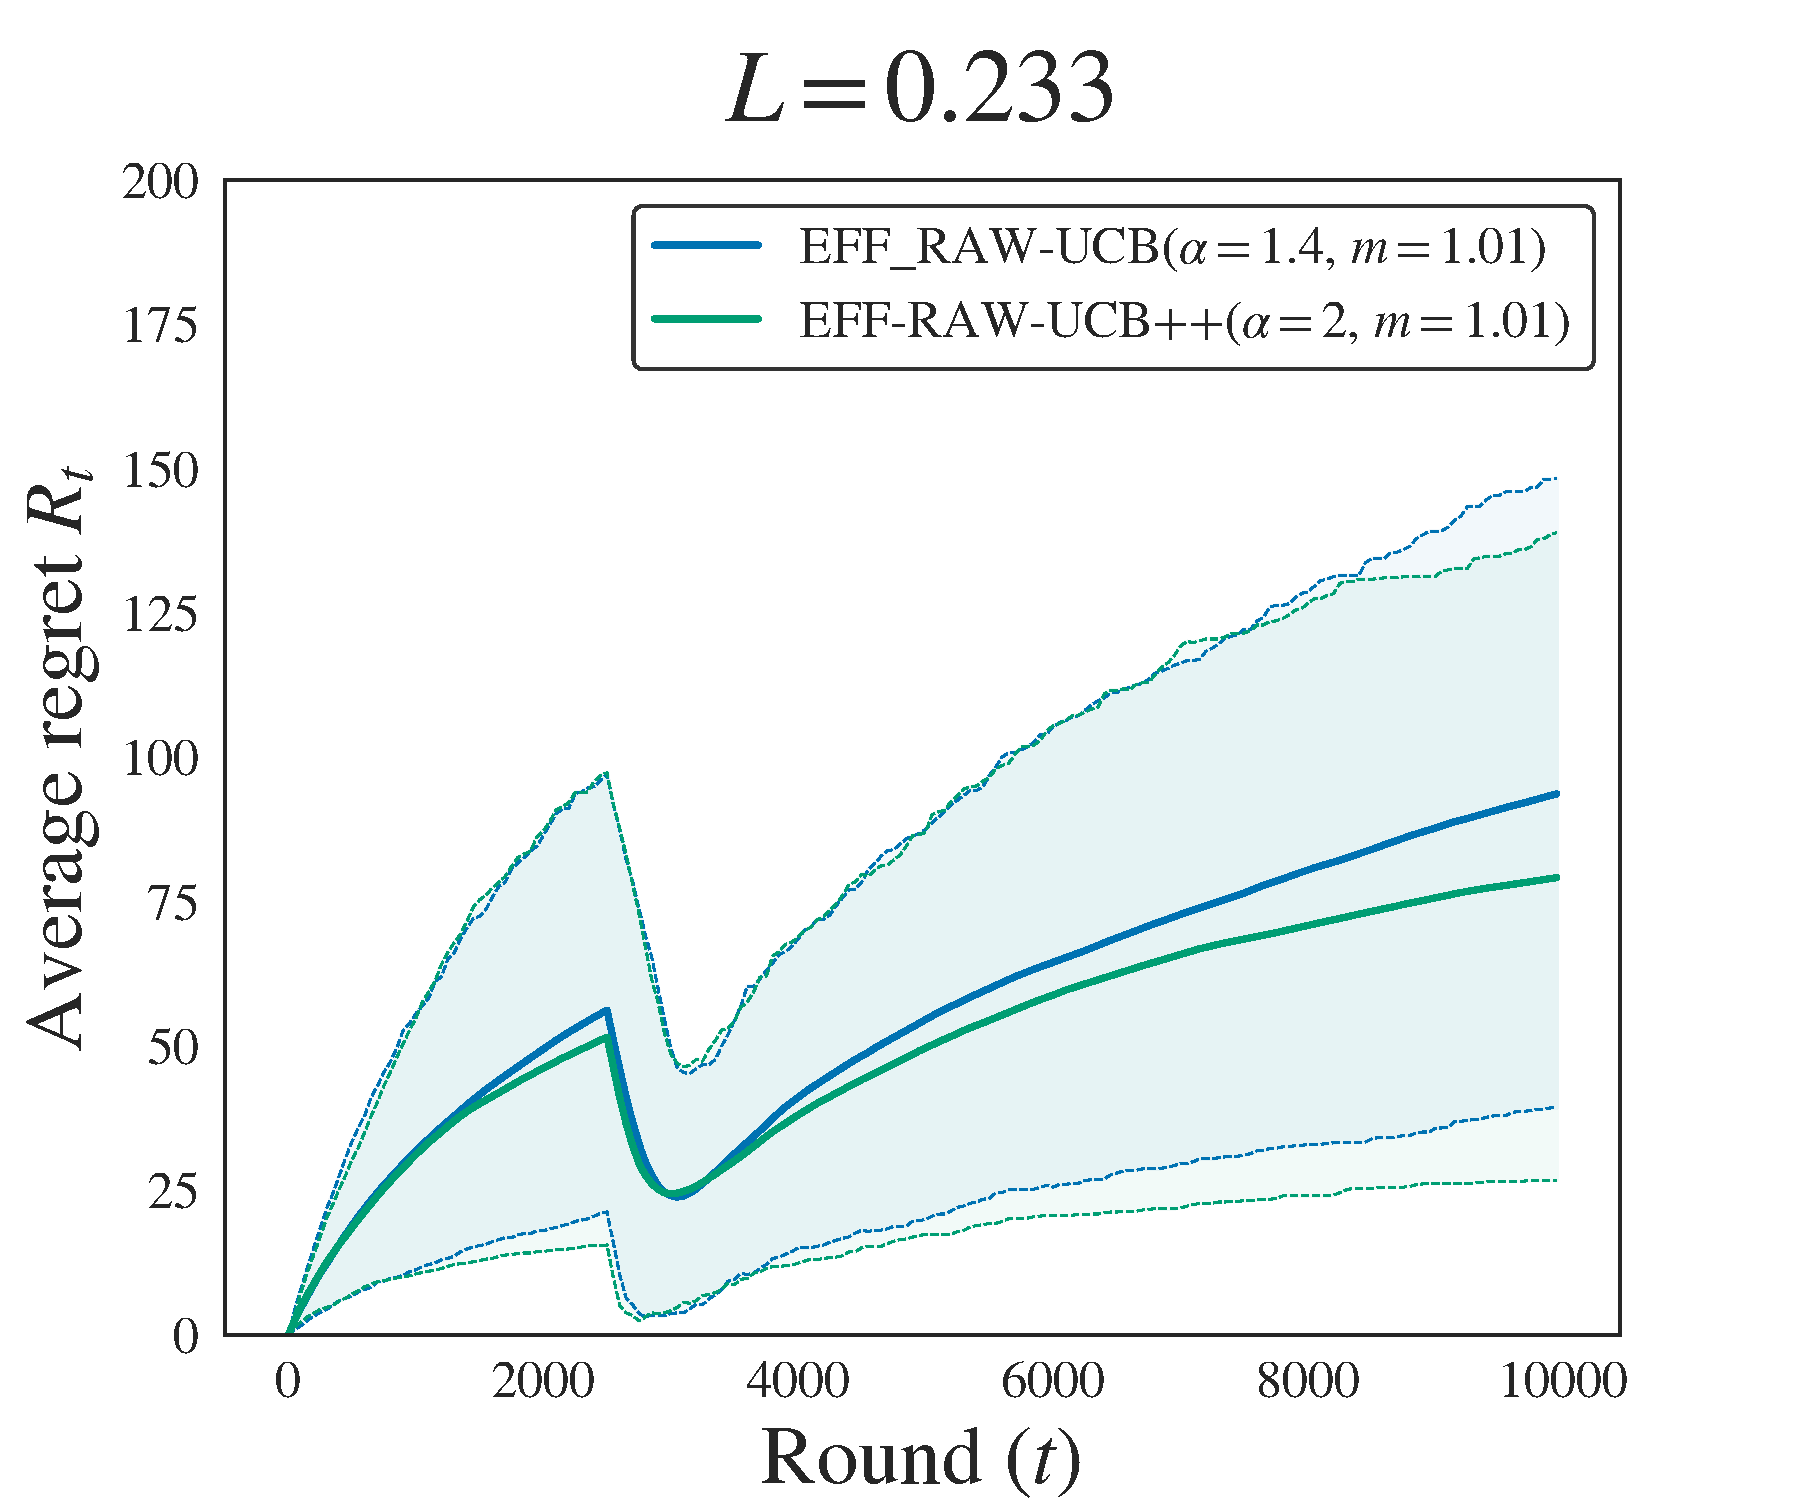
\includegraphics[clip, width= 0.49\textwidth]{2.1Rested/fig/fig1B_pp.pdf}
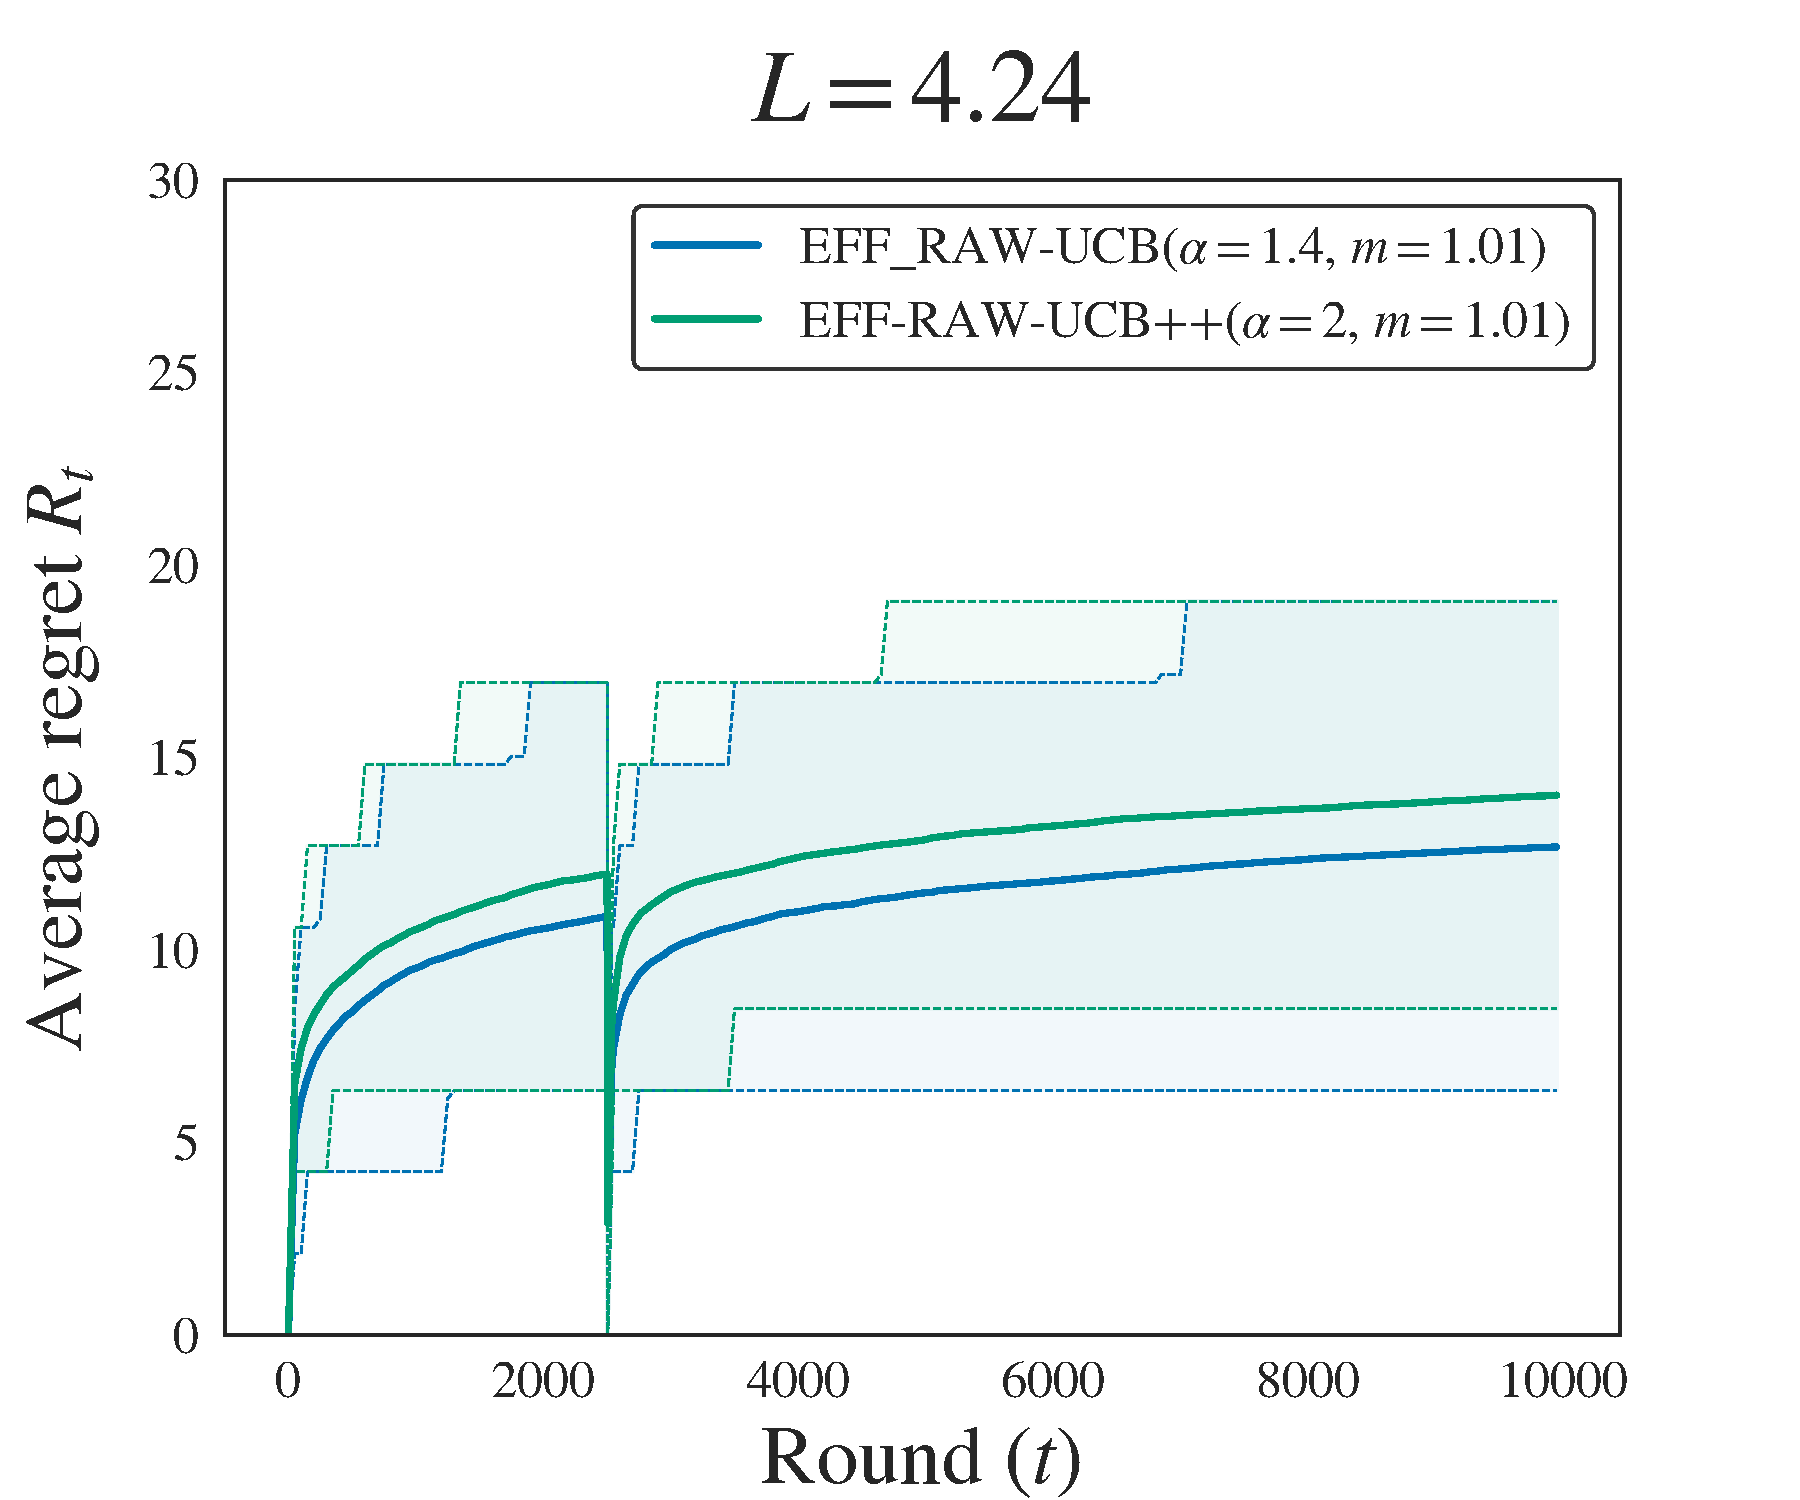
\includegraphics[clip, width= 0.49\textwidth]{2.1Rested/fig/fig1C_pp.pdf}
\caption{\textbf{Top:} Regret at the end of the game for different values of $L$. \textbf{Bottom:} Regret across time for two values of $L$. Average over 1000 runs. We highlight the $\left[10\%, 90\%\right]$ confidence region.}
\label{fig:rested-pp1}
\end{figure*}


\begin{figure*}[ht]
\centering
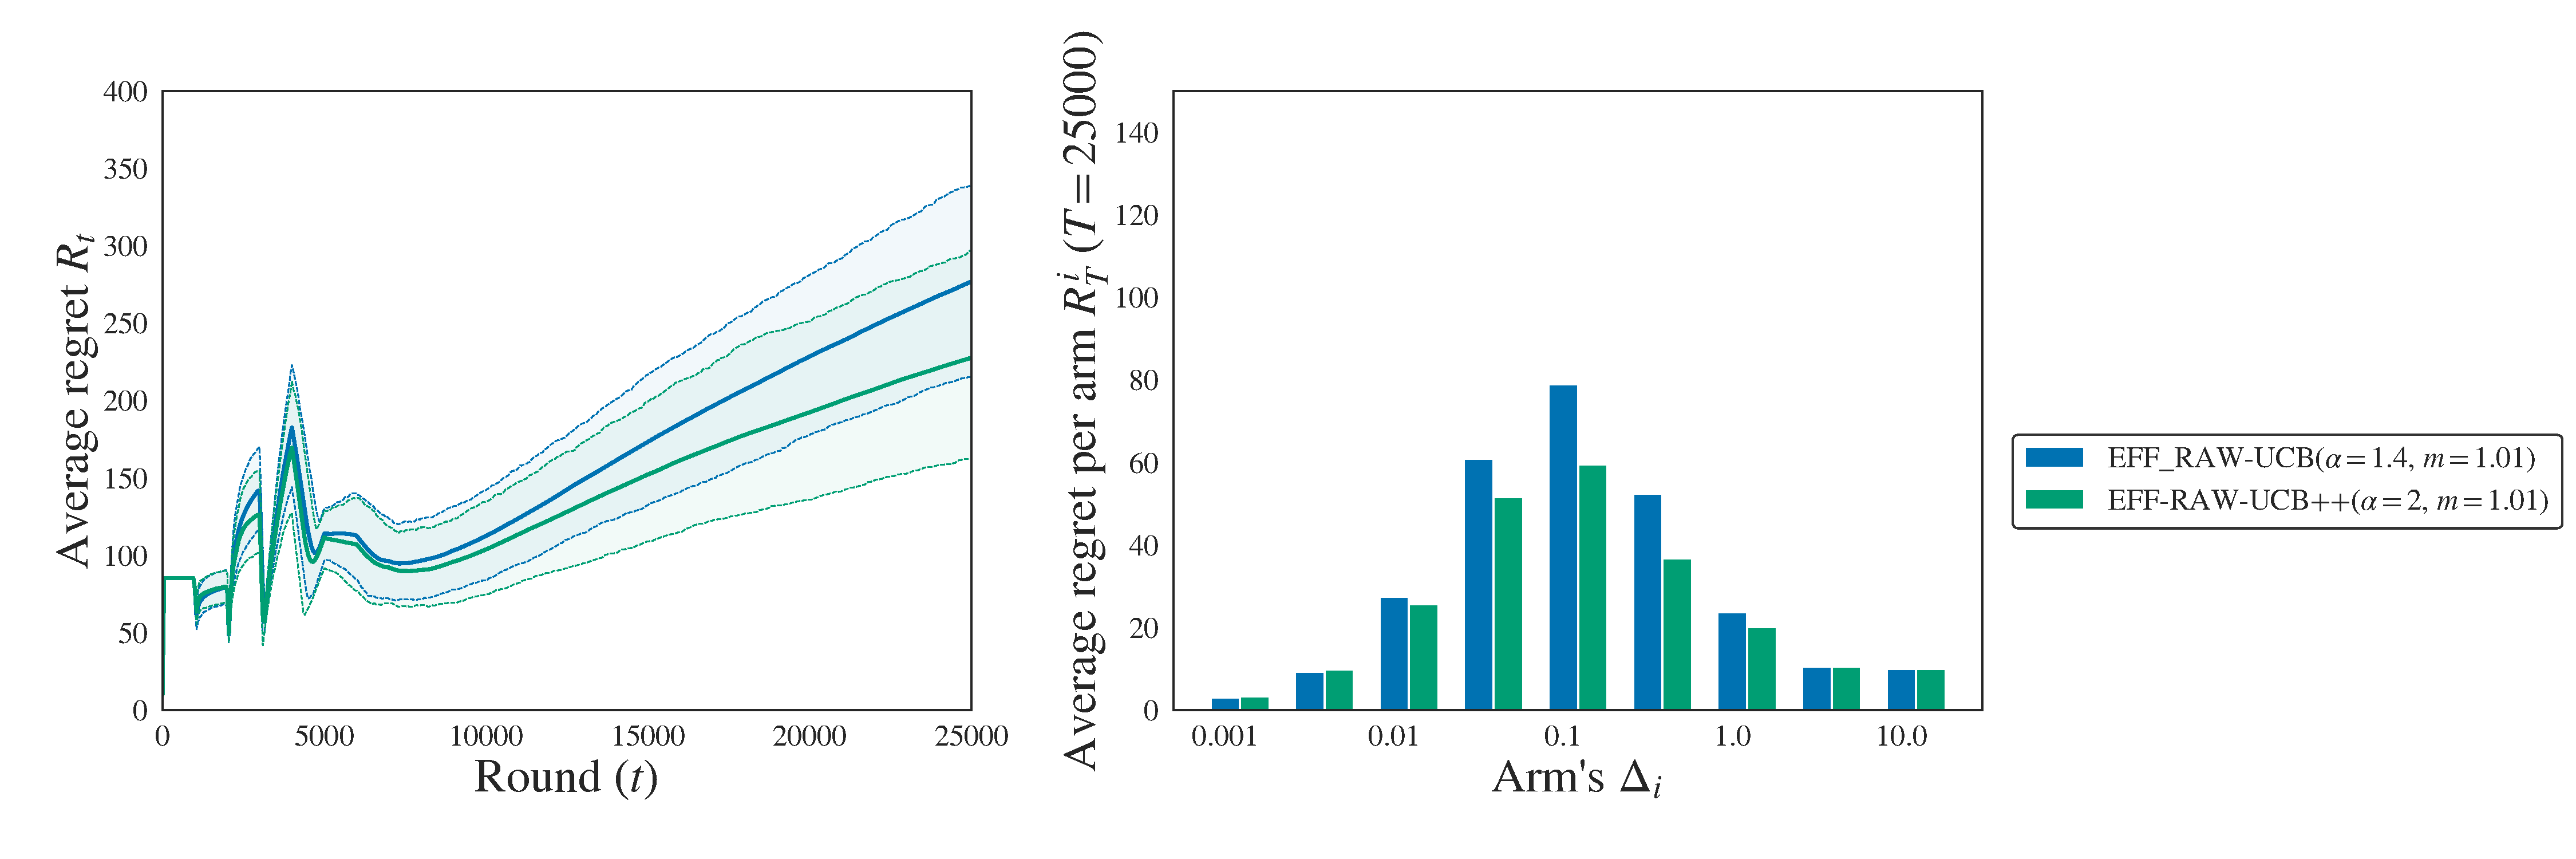
\includegraphics[width = 0.99 \textwidth]{2.1Rested/fig/fig2_pp.pdf}
\caption{\textbf{Left:} Regret at the end of the game for different values of $L$. \textbf{Middle, Right:} Regret across time for two values of $L$. Average over 1000 runs. We highlight the $\left[10\%, 90\%\right]$ confidence region.}
\label{fig:rested-pp2}
\end{figure*}

\subsection{Towards a theoretical analysis of {\RAWUCBpp}}
Analyzing \UCB with tight confidence levels in stationary bandits is already a challenging task \citep{degenne2016anytime, menard2017klucb++, lattimore2018refining}. The analysis of \RAWUCBpp faces two additional difficulties: on the one hand, \RAWUCB 's meta-index is more complex than \UCB 's; on the other hand, rotting bandits are more difficult to analyze than stationary ones. 

First, we can ignore the second part of the problem and try to analyze \RAWUCBpp on stationary problems. Tight analysis of \UCB usually bound the number of pulls of the suboptimal arms. A classical trick is to set a threshold $\mu_\star - \epsilon_i$ and notice that a necessary condition to pull a suboptimal arm $i$ is that either the index of the optimal arm is below the threshold, or the index of the suboptimal arm is above the threshold,

\[ \NiT \leq \sum_{t=1}^T \1 \left[ \texttt{ind}\pa{i_\star, t, \delta_{t,h}} < \mu_\star - \epsilon_i \right] + \1 \left[ \texttt{ind}\pa{i, t, \delta_{t,h}} > \mu_\star - \epsilon_i \right].
\]

The upper deviation of suboptimal arms' indexes is not more difficult to control for \RAWUCB than for \UCB. Indeed, since we take the minimum across confidence bounds, the indexes of \RAWUCB are smaller than the indexes of \UCB (when the confidence levels are the same). 

Controlling the lower deviation of the optimal arm's index is more challenging.  Indeed, at each round $t$, we have to control the probability that any ucb associated with any $h$ last pulls after any $N_{i,t}$ pulls is below the threshold. Compared to \UCB where there is only a scan on the possible values of $N_{i,t}$, we have to handle a double scan on $N_{i,t}$ and $h$. In Section~\ref{sec:theory}, we handle the multiple windows with a crude union bound which leads to a fairly large decrease of the confidence levels. A tighter analysis would probably require better statistical engineering than a union bound or a simple peeling argument. For instance, \citet{maillard2019sequential} develop new concentration results for similar scan statistics for sequential change-point detectors (with some applications to bandits). The difficulty is that the quantity to be bounded is not a sub/super-martingale. Yet, it is quite uncertain that a tighter analysis is actually possible in our case. Indeed, the empirical tuning of \RAWUCB (resp. \RAWUCBpp) increases $\alpha$ by 0.4 (resp. 1) compared to the confidence levels of \UCB (resp. \MOSSa). This is comparable with the theoretical increase of $1$ due to the union bound over all the possible windows.